%%%%%%%%%%%%%%%%%%%%%%%%%%%%%%%%%%%%%%%%%%%%%%%%%%%%%%%%%%%%%%%%%%%%%%%%%%%%%%%%%%
\begin{frame}[fragile]\frametitle{}
\begin{center}
{\Large Deploy Your Own Model}
\end{center}
\end{frame}

%%%%%%%%%%%%%%%%%%%%%%%%%%%%%%%%%%%%%%%%%%%%%%%%%%%%%%%%%%
\begin{frame}[fragile]\frametitle{What is MLOps?}
\adjustbox{valign=t}{%
\begin{minipage}{0.56\linewidth}
\begin{itemize}
\item MLOps: the practices for building, deploying, monitoring and updating ML systems reliably
\item A trained model is not the end: the loop keeps running
\item Example for this section: predict the city MPG of a car from its engine size, horsepower and weight
\end{itemize}
\end{minipage}%
}%
\hfill%
\adjustbox{valign=t}{%
\begin{minipage}{0.4\linewidth}
\begin{center}
\adjustbox{max width=\linewidth, max totalheight=4cm}{%
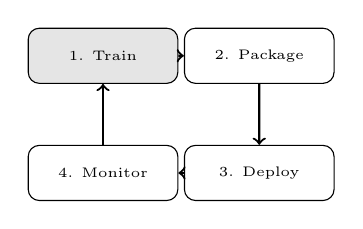
\begin{tikzpicture}[scale=0.62, every node/.style={font=\tiny}]
\node[draw, rounded corners, minimum width=1.9cm, minimum height=0.7cm, fill=gray!20] (a) at (0,2.4) {1. Train};
\node[draw, rounded corners, minimum width=1.9cm, minimum height=0.7cm] (b) at (3.2,2.4) {2. Package};
\node[draw, rounded corners, minimum width=1.9cm, minimum height=0.7cm] (c) at (3.2,0) {3. Deploy};
\node[draw, rounded corners, minimum width=1.9cm, minimum height=0.7cm] (d) at (0,0) {4. Monitor};
\draw[->, thick] (a) -- (b);
\draw[->, thick] (b) -- (c);
\draw[->, thick] (c) -- (d);
\draw[->, thick] (d) -- (a);
\end{tikzpicture}%
}
\end{center}
\tiny{The MLOps loop: monitoring feeds back into retraining.}
\end{minipage}%
}
\end{frame}

%%%%%%%%%%%%%%%%%%%%%%%%%%%%%%%%%%%%%%%%%%%%%%%%%%%%%%%%%%
\begin{frame}[fragile]\frametitle{Step 1: Save the Trained Model}
\begin{itemize}
\item Train once; the service only needs the saved model
\item \texttt{joblib} stores the fitted model, with everything it learned
\item Only load model files you trust: like pickle, joblib can run code while loading
\end{itemize}
\begin{lstlisting}
from sklearn.ensemble import RandomForestRegressor
import joblib

# X: engine size, horsepower, weight of each car; y: city MPG
model = RandomForestRegressor(n_estimators=100, random_state=0).fit(X, y)
joblib.dump(model, 'mpg_model.joblib')        # save

# In the Python shell (a new session):
>>> import joblib
>>> model = joblib.load('mpg_model.joblib')
>>> print(model.predict([[2.0, 140, 2800]]).round(1))
[24.5]
\end{lstlisting}
\end{frame}

%%%%%%%%%%%%%%%%%%%%%%%%%%%%%%%%%%%%%%%%%%%%%%%%%%%%%%%%%%
\begin{frame}[fragile]\frametitle{Step 2: Serve It as an API}
\begin{itemize}
\item An API lets any program call the model over HTTP
\item FastAPI checks each request against the \texttt{Car} type: wrong types are rejected with HTTP 422
\end{itemize}
\begin{lstlisting}
# app.py     (run it with:  uvicorn app:app --port 8000)
from fastapi import FastAPI
from pydantic import BaseModel
import joblib

model = joblib.load("mpg_model.joblib")     # load once, at start-up
app = FastAPI()

class Car(BaseModel):
    engine_size: float
    horsepower: float
    weight: float

@app.post("/predict")
def predict(car: Car):
    x = [[car.engine_size, car.horsepower, car.weight]]
    return {"mpg_city": round(float(model.predict(x)[0]), 1)}
\end{lstlisting}
\end{frame}

%%%%%%%%%%%%%%%%%%%%%%%%%%%%%%%%%%%%%%%%%%%%%%%%%%%%%%%%%%
\begin{frame}[fragile]\frametitle{Step 3: Call the Service}
\begin{itemize}
\item Send the features as JSON; the service answers with JSON
\item Any language or tool can be the client: a web page, a PLC gateway, a spreadsheet macro
\item Test the bad-input case too: a text value for \texttt{engine\_size} returns HTTP 422
\end{itemize}
\begin{lstlisting}
$ curl -X POST http://localhost:8000/predict \
       -H "Content-Type: application/json" \
       -d '{"engine_size": 2.0, "horsepower": 140, "weight": 2800}'
{"mpg_city":24.5}
\end{lstlisting}
\end{frame}

%%%%%%%%%%%%%%%%%%%%%%%%%%%%%%%%%%%%%%%%%%%%%%%%%%%%%%%%%%
\begin{frame}[fragile]\frametitle{Step 4: Package It in a Container}
\begin{itemize}
\item A container bundles the code, the model and the libraries: it runs the same on a laptop and on a cloud server
\item Pin library versions in \texttt{requirements.txt}: load the model with the same scikit-learn version that saved it
\item Then run the image on a cloud server (for example an AWS EC2 instance) or any container service
\end{itemize}
\begin{lstlisting}
# Dockerfile
FROM python:3.11-slim
WORKDIR /app
COPY requirements.txt .
RUN pip install -r requirements.txt
COPY app.py mpg_model.joblib ./
CMD ["uvicorn", "app:app", "--host", "0.0.0.0", "--port", "8000"]
\end{lstlisting}
\end{frame}

%%%%%%%%%%%%%%%%%%%%%%%%%%%%%%%%%%%%%%%%%%%%%%%%%%%%%%%%%%
\begin{frame}[fragile]\frametitle{Step 5: Monitor and Retrain}
\begin{itemize}
\item Models degrade when the world changes
\begin{itemize}
\item Data drift: the inputs no longer look like the training data
\item Concept drift: the relation between inputs and output changes
\end{itemize}
\item Monitor input statistics, prediction quality (when true values arrive), latency and errors
\item When drift is flagged: retrain on newer data, version the new model file, redeploy
\item The KS test (\texttt{ks\_2samp}) asks whether two samples come from the same distribution: a small p-value means they differ
\end{itemize}
\begin{lstlisting}
from scipy.stats import ks_2samp

# train_weight: weights in the training data
# new_ok, new_heavy: last week's requests, and a batch with 20% heavier cars
>>> print(ks_2samp(train_weight, new_ok).pvalue.round(3))
0.693
>>> print(ks_2samp(train_weight, new_heavy).pvalue < 0.01)
True
\end{lstlisting}
\end{frame}

%%%%%%%%%%%%%%%%%%%%%%%%%%%%%%%%%%%%%%%%%%%%%%%%%%%%%%%%%%
\begin{frame}[fragile]\frametitle{Quick Check: Model Drift}
\begin{block}{Think About It}
The MPG service was accurate at launch. Six months later most requests are for a new range of heavier hybrid cars, and accuracy has fallen, although the code has not changed. What is the most likely cause, and the right response?
\begin{enumerate}
  \item[A.] A bug in the API code: redeploy the same model
  \item[B.] Data drift: the inputs no longer match the training data; detect it by monitoring inputs, then retrain on newer data and redeploy
  \item[C.] joblib files expire after six months: save the model file again
  \item[D.] The server is too slow: buy a bigger cloud server
\end{enumerate}
\end{block}
\end{frame}

%%%%%%%%%%%%%%%%%%%%%%%%%%%%%%%%%%%%%%%%%%%%%%%%%%%%%%%%%%%%%%%%%%%%%%%%%%%%%%%%%%
\begin{frame}[fragile]\frametitle{Quick Check: Model Drift}
\begin{block}{Answer}
\textbf{Correct: B.} The model still answers as before, but it now sees cars unlike those it was trained on, so its accuracy falls. Unchanged code rules out a bug (A), a saved file does not expire (C), and a bigger server changes speed, not accuracy (D). Monitoring the inputs (for example with a drift test) is what reveals the problem.
\end{block}
\end{frame}
